\documentclass[a4paper, fontsize = 14pt]{article}
\usepackage{hyperref}
\usepackage[warn]{mathtext}
\usepackage[english,russian]{babel}
\usepackage[utf8x]{inputenc} 
 
%математика
\usepackage[mathscr]{eucal}
\usepackage{amsmath,amsfonts,amssymb,amsthm,mathtools}
\usepackage{icomma}
\usepackage{wasysym}
\usepackage{mathrsfs}
 
%оформление текста
\usepackage{setspace}
\onehalfspacing
\usepackage{indentfirst}
\usepackage{scrextend}
 
%геометрия
\usepackage{geometry}4241
\geometry{left=25mm,right=25mm,
 top=25mm,bottom=30mm}
 
%графика
\usepackage{wrapfig}
\usepackage{graphicx}
\usepackage{pgfplots}
\usepackage{tikz}
\usepackage{hvfloat}
\RequirePackage{caption}
\DeclareCaptionLabelSeparator{defffis}{ --- }
\captionsetup{justification=centering,labelsep=defffis}
 
%таблицы
\usepackage{array,tabularx,tabulary,booktabs} 
\usepackage{longtable}  
\usepackage{multirow} 
 
%ссылки
\usepackage{hyperref}
\usepackage{xcolor}
\definecolor{grn}{HTML}{57A14F} %зеленый
\definecolor{rd}{HTML}{E53C44} %красный 
\definecolor{bl}{HTML}{282691} %синий 
\definecolor{bbl}{HTML}{001B6C} %темно-синий
\hypersetup{		
    colorlinks=true,       	
    linkcolor=bbl,          % внутренние ссылки
    citecolor=rd,          % на библиографию
    filecolor=magenta,      % на файлы
    urlcolor=bl           %внешние источники
}
 
% Колонтитулы
\usepackage{fancyhdr} 
 	\pagestyle{fancy}
 	\renewcommand{\headrulewidth}{0.15mm}  
 	\renewcommand{\footrulewidth}{0.15mm}
 	\lfoot{МФТИ, 2021}
 	\rfoot{\thepage}
 	\cfoot{}
 	\rhead{}
 	\chead{}
 	\lhead{}
 
 
\begin{document}
 
\begin{center} \large\textbf{
Лабораторная работа №2.2.1 \\ Исследование взаимной диффузии газов \\
Мещеряков Всеволод, Б02-001, 05.03.2021}
\end{center} 

\subsection*{Введение}

Цель работы: определение коэффициента взаимной диффузии гелия и воздуха.

\subsection*{Экспериментальная установка}

\begin{figure}[hbt]
\center{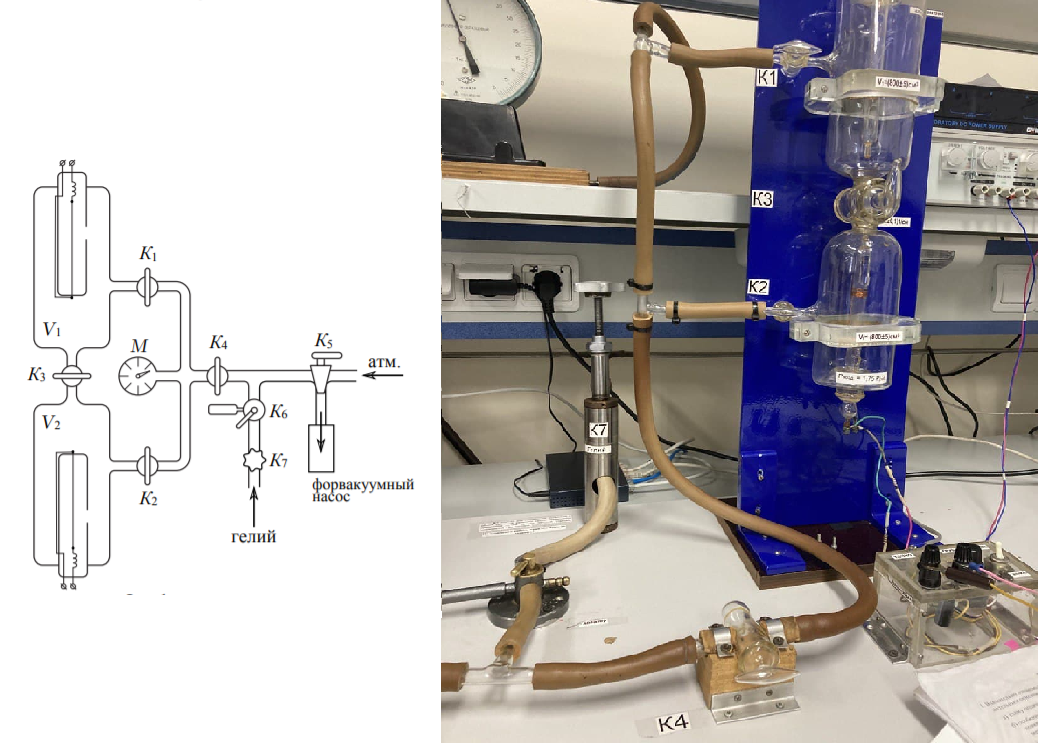
\includegraphics[scale=0.65]{lab221ris1.png}}
\caption{\textit{Схема и фотография установки}}
\end{figure}

Работа проводилась на установке, схема и фотография которой изображены на рисунке 1. На схеме: 

\begin{itemize}
  \item К1 - кран, перекрывающий верхний сосуд $V_1$, в который будет нагнетаться гелий;
  \item К2 - подвижная перегородка, соединяющая сосуды $V_1$ и $V_2$, через которую и будут смешиваться газы;
  \item К3 - кран, перекрывающий нижний сосуд $V_2$, в который будет нагнетаться воздух;
  \item К4 - кран, соединяющий сосуды с форвакуумным насосом;
  \item К5 - кран, контролирующий откачку/закачку воздуха из сосудов;	  \item К6 - кран, соединяющий сосуды с баллоном, содержащим гелий;
  \item К7 - кран баллона, содержащего гелий.
\end{itemize}

Параметры установки: \[ V_1=V_2=(800\pm5)\,см^3 \, , L/S=(15,0\pm0,1) \, см^{-1} \, , P_{атм}=724 \, торр \, . \]

\subsection*{Ход работы}

Каждое измерение сопровождается подготовкой установки к работе.

Откачаем воздух из системы:

\begin{enumerate}
	\item Откроем К4, чем откроем сосуды;
	\item Включим форвакуумный насос;
	\item Откроем К5, чем соединим насос с сосудами;
	\item Дожидаемся $\approx 0,1 \,\, торр$ на манометре, после чего перекрываем К5 и изолируем сосуды.
\end{enumerate}

Заполним установку воздухом до рабочего давления. Цену деления манометра интерпретируем под текущее атмосферное давление:

\[ P_0 = \frac{ 724 \, торр }{100 \, делений} = 7,24 \, торр / деление.\]

Первое измерение проведем при $3,5 P_0  \approx 25,34 \, торр $. Добьемся этого, слабо повернув К5, запустив в систему некоторое количество воздуха. После сбалансируем мост, добившись на нем нулевого значения.

Затем напустим в сосуд $V_1$ гелия согласно указаниям. Контроллировать количество вещества будем с помощью манометра, который будет подключен к $V_1$. 

Изолируем сосуды, закрыв К1 и К2, и запустим процесс диффузии, открыв К3. Вместе с открытием К3 запускаем секундомер и начинаем снимать зависимость напряжения на мосте от времени. Записываем показания каждые 10 секунд до тех пор, пока снимаемая величина не упадет до $30-40\%$ от исходной. 

\subsection*{Измерения}

Проведем измерения для разных давлений, каждому измерению предшествует подготовка, описанная параграфом выше. Результаты отражены в таблицах 1, 2, 3, приложения. Для каждого из давлений построим графики на осях времени и логарифма показаний вольтметра. Из каждого графика по наклону прямой определяем коэффициент. 

\subsection*{Обработка результатов}

Из теории имеем, что разность концентраций будет убывать по экспоненциальному закону. Отсюда следует, что и показания вольтметра будут изменяться так же:

\[ U = U_0 e^{-t/\tau} .\]

В формуле выше $U_0$ - начальное показание вольтметра, U - показания вольтметра в момент времени t, t - время от начала процесса, $\tau$ - характерное время, определяемое формулой (1):

\begin{equation}
	\tau = \frac{V_1 V_2}{V_1+V_2} \frac{l}{SD}.
\end{equation}

Отсюда получаем, что измеренные данные из таблиц 1, 2, 3 можно представить в виде линейной зависимости (см. Рис2 приложения), коэффициент наклона которой позволит вычислить искомую величину D:

\begin{equation}
	\-ln{\frac{U(t)}{U_0}}=k\cdot t. \underset{формула (1)}{\Rightarrow} D=k\frac{Vl}{2S}.  
\end{equation}

Из полученных по МНК графиков вычисляем k для каждого из давлений:
\[ k_{25торр}=(41,1\pm0,2)\cdot 10^{-4}(1/с) \underset{(2)}{\Rightarrow} D_{25торр}=(24,6\pm1,2)(см^2/c) \]
\[ k_{40торр}=(21,7 \pm0,8)\cdot 10^{-4}(1/с) \underset{(2)}{\Rightarrow} D_{40торр}(13,0\pm1,5)(см^2/c) \]
\[ k_{70торр}=(16,4\pm0,8)\cdot 10^{-4}(1/с) \underset{(2)}{\Rightarrow} D_{70торр} =(9,84\pm1,4)(см^2/c) \]

Тогда можем экстраполировать зависимость $D(\frac{1}{P})$, из которой увидим значение искомого коэффициента при атмосферном давлении:

\[ D_{атм} = (79\pm14)\cdot 10^{-2} (см^2/c), \, \varepsilon_{D_атм} = 18\% \]
\[ D_{атм} = 57 \cdot 10^{-2} (см^2/c) \, - табличное \, \, \, значение. \]

\subsection*{Приложение}

\begin{table}[h]
\centering
\caption{U(t) при давлении $3,5P_0=25 \, торр$}
\begin{tabular}{|l|c|c|c|c|c|c|c|c|c|c|}
\hline
\textbf{t, сек} & \textbf{0}   & \textbf{10}  & \textbf{20}  & \textbf{30}  & \textbf{40}  & \textbf{50}  & \textbf{60}  & \textbf{70}  & \textbf{80}  & \textbf{90}  \\ \hline
\textbf{U, мВ}  & 0,86         & 0,84         & 0,81         & 0,78         & 0,75         & 0,72         & 0,69         & 0,67         & 0,64         & 0,62         \\ \hline
\textbf{t, сек} & \textbf{100} & \textbf{110} & \textbf{120} & \textbf{130} & \textbf{140} & \textbf{150} & \textbf{160} & \textbf{170} & \textbf{180} & \textbf{190} \\ \hline
\textbf{U, мВ}  & 0,59         & 0,57         & 0,55         & 0,52         & 0,50         & 0,48         & 0,46         & 0,45         & 0,43         & 0,41         \\ \hline
\textbf{t, сек} & \textbf{200} & \textbf{210} & \textbf{220} & \textbf{230} & \textbf{240} & \textbf{250} & \textbf{260} & \textbf{270} & \textbf{280} & \textbf{290} \\ \hline
\textbf{U, мВ}  & 0,38         & 0,37         & 0,36         & 0,34         & 0,33         & 0,31         & 0,30         & 0,29         & 0,28         & 0,27         \\ \hline
\end{tabular}
\end{table}

\begin{table}[h]
\centering
\caption{U(t) при давлении $5,5P_0=40 \, торр$}
\begin{tabular}{|l|c|c|c|c|c|c|c|c|c|c|}
\hline
\textbf{t, сек} & \textbf{0}   & \textbf{10}  & \textbf{20}  & \textbf{30}  & \textbf{40}  & \textbf{50}  & \textbf{60}  & \textbf{70}  & \textbf{80}  & \textbf{90}  \\ \hline
\textbf{U, мВ}  & 1,14         & 1,13         & 1,11         & 1,08         & 1,06         & 1,04         & 1,02         & 1,00         & 0,98         & 0,96         \\ \hline
\textbf{t, сек} & \textbf{100} & \textbf{110} & \textbf{120} & \textbf{130} & \textbf{140} & \textbf{150} & \textbf{160} & \textbf{170} & \textbf{180} & \textbf{190} \\ \hline
\textbf{U, мВ}  & 0,94         & 0,92         & 0,90         & 0,88         & 0,86         & 0,84         & 0,82         & 0,80         & 0,78         & 0,76         \\ \hline
\textbf{t, сек} & \textbf{200} & \textbf{210} & \textbf{220} & \textbf{230} & \textbf{240} & \textbf{250} & \textbf{260} & \textbf{270} & \textbf{280} & \textbf{290} \\ \hline
\textbf{U, мВ}  & 0,74         & 0,72         & 0,71         & 0,69         & 0,68         & 0,66         & 0,64         & 0,63         & 0,62         & 0,61         \\ \hline
\textbf{t, сек} & \textbf{300} & \textbf{310} & \textbf{320} & \textbf{330} & \textbf{340} & \textbf{350} & \textbf{360} & \textbf{370} & \textbf{380} & \textbf{390} \\ \hline
\textbf{U, мВ}  & 0,59         & 0,58         & 0,57         & 0,56         & 0,54         & 0,53         & 0,52         & 0,51         & 0,50         & 0,49         \\ \hline
\textbf{t, сек} & \textbf{400} & \textbf{410} & \textbf{420} & \textbf{430} & \textbf{440} & \textbf{450} & \textbf{460} & \textbf{470} & \textbf{480} & \textbf{490} \\ \hline
\textbf{U, мВ}  & 0,48         & 0,47         & 0,46         & 0,45         & 0,44         & 0,43         & 0,42         & 0,41         & 0,40         & 0,40         \\ \hline
\textbf{t, сек} & \textbf{500} & \textbf{510} & \textbf{520} & \textbf{530} & \textbf{540} & \textbf{550} & \textbf{560} & \textbf{570} & \textbf{580} & \textbf{590} \\ \hline
\textbf{U, мВ}  & 0,39         & 0,38         & 0,38         & 0,37         & 0,36         & 0,35         & 0,34         & 0,34         & 0,33         & 0,32         \\ \hline
\textbf{t, сек} & \textbf{600} & \textbf{610} & \textbf{620} &              &              &              &              &              &              &              \\ \hline
\textbf{U, мВ}  & 0,32         & 0,31         & 0,31         &              &              &              &              &              &              &              \\ \hline
\end{tabular}
\end{table}

\begin{table}[h]
\centering
\caption{U(t) при давлении $9,5P_0=70 \, торр$}
\begin{tabular}{|l|c|c|c|c|c|c|c|c|c|c|}
\hline
\textbf{t, сек} & \textbf{0}   & \textbf{10}  & \textbf{20}  & \textbf{30}  & \textbf{40}  & \textbf{50}  & \textbf{60}  & \textbf{70}  & \textbf{80}  & \textbf{90}  \\ \hline
\textbf{U, мВ}  & 2,29         & 2,26         & 2,23         & 2,19         & 2,16         & 2,12         & 2,09         & 2,05         & 2,02         & 1,99         \\ \hline
\textbf{t, сек} & \textbf{100} & \textbf{110} & \textbf{120} & \textbf{130} & \textbf{140} & \textbf{150} & \textbf{160} & \textbf{170} & \textbf{180} & \textbf{190} \\ \hline
\textbf{U, мВ}  & 1,95         & 1,92         & 1,89         & 1,85         & 1,82         & 1,80         & 1,77         & 1,74         & 1,70         & 1,68         \\ \hline
\textbf{t, сек} & \textbf{200} & \textbf{210} & \textbf{220} & \textbf{230} & \textbf{240} & \textbf{250} & \textbf{260} & \textbf{270} & \textbf{280} & \textbf{290} \\ \hline
\textbf{U, мВ}  & 1,65         & 1,62         & 1,60         & 1,56         & 1,54         & 1,52         & 1,49         & 1,46         & 1,44         & 1,42         \\ \hline
\textbf{t, сек} & \textbf{300} & \textbf{310} & \textbf{320} & \textbf{330} & \textbf{340} & \textbf{350} & \textbf{360} & \textbf{370} & \textbf{380} & \textbf{390} \\ \hline
\textbf{U, мВ}  & 1,39         & 1,37         & 1,35         & 1,32         & 1,30         & 1,28         & 1,25         & 1,24         & 1,22         & 1,18         \\ \hline
\textbf{t, сек} & \textbf{400} & \textbf{410} & \textbf{420} & \textbf{430} & \textbf{440} & \textbf{450} & \textbf{460} & \textbf{470} & \textbf{480} & \textbf{490} \\ \hline
\textbf{U, мВ}  & 1,18         & 1,16         & 1,14         & 1,12         & 1,10         & 1,09         & 1,07         & 1,05         & 1,03         & 1,02         \\ \hline
\textbf{t, сек} & \textbf{500} & \textbf{510} & \textbf{520} & \textbf{530} & \textbf{540} & \textbf{550} & \textbf{560} & \textbf{570} & \textbf{580} & \textbf{590} \\ \hline
\textbf{U, мВ}  & 1,00         & 0,99         & 0,98         & 0,97         & 0,95         & 0,94         & 0,93         & 0,92         & 0,91         & 0,91         \\ \hline
\end{tabular}
\end{table}

\centering
\hvFloat[floatPos=htb, capWidth=h, capPos=r, capAngle=90, objectAngle=90, capVPos=c, objectPos=c]{figure}{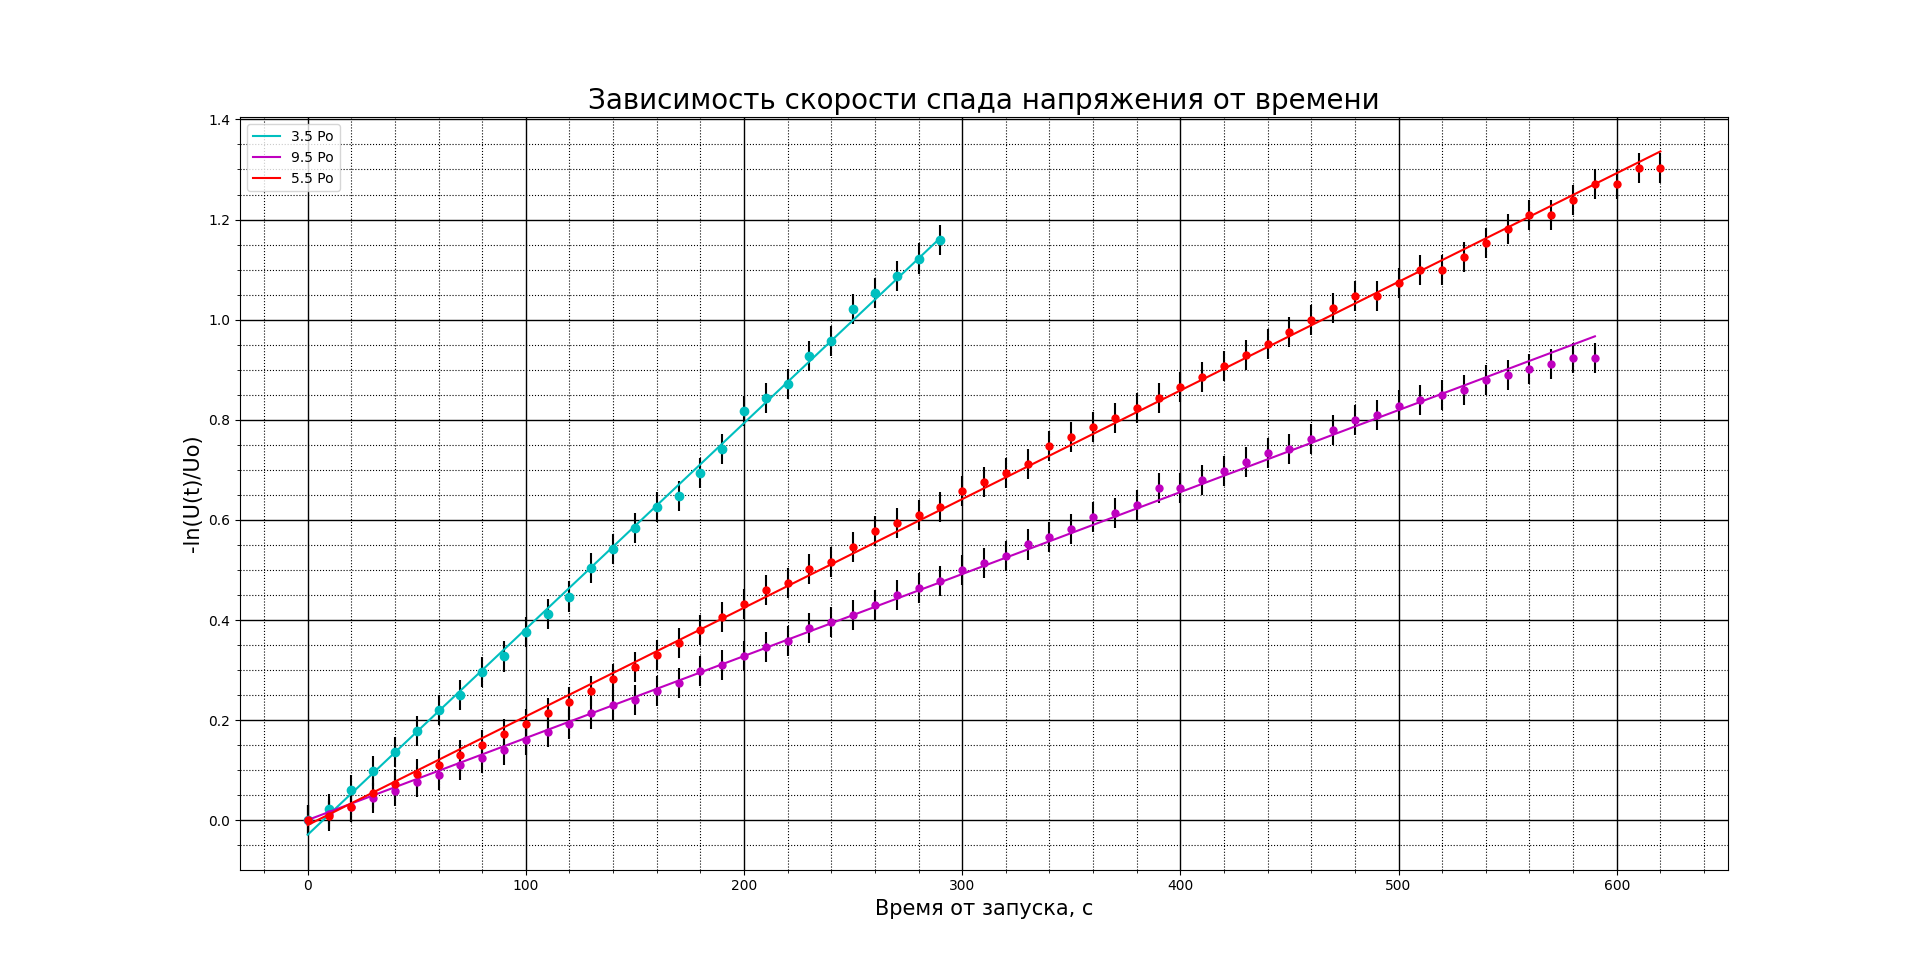
\includegraphics[scale=0.55]{lab221ris2.png}}
{\textit{Графики зависимости $-ln{\frac{U}{U_0}}(t)$ при разных начальных давлениях}}{fig:fig2}






\end{document}